\chapter{Perceptual Grouping}\label{chapter:perceptual_organization}
\index{Perceptual grouping}

\section{Introduction}

The previous chapter discussed the importance of learning good visual representations, which can serve as the substrate for further vision algorithms. In this chapter we will continue our exploration of perceptual representations, but we will approach it from a slightly different school of thought, which is inherited from pre-deep learning computer vision and from human vision science. In this tradition, one particular kind of visual representation, the \index{Perceptual grouping}\textbf{perceptual group}, becomes the central object of interest; we will see what these are, how to find them, and how they are related to the representation learning algorithms from the last chapter.

First, what is a perceptual group? Look at the photo in \fig{\ref{fig:perceptual_organization:perc_org_teaser}} and consider what you see. Not what raw pixel values you see, but what structures you see. What are some structures you can name?
%We humans see the world as organized into different levels of perceptual structure: contours and surfaces, objects and events (\fig{\ref{fig:perceptual_organization:perc_org_teaser}}).
\begin{figure}[h!]
    \centerline{
        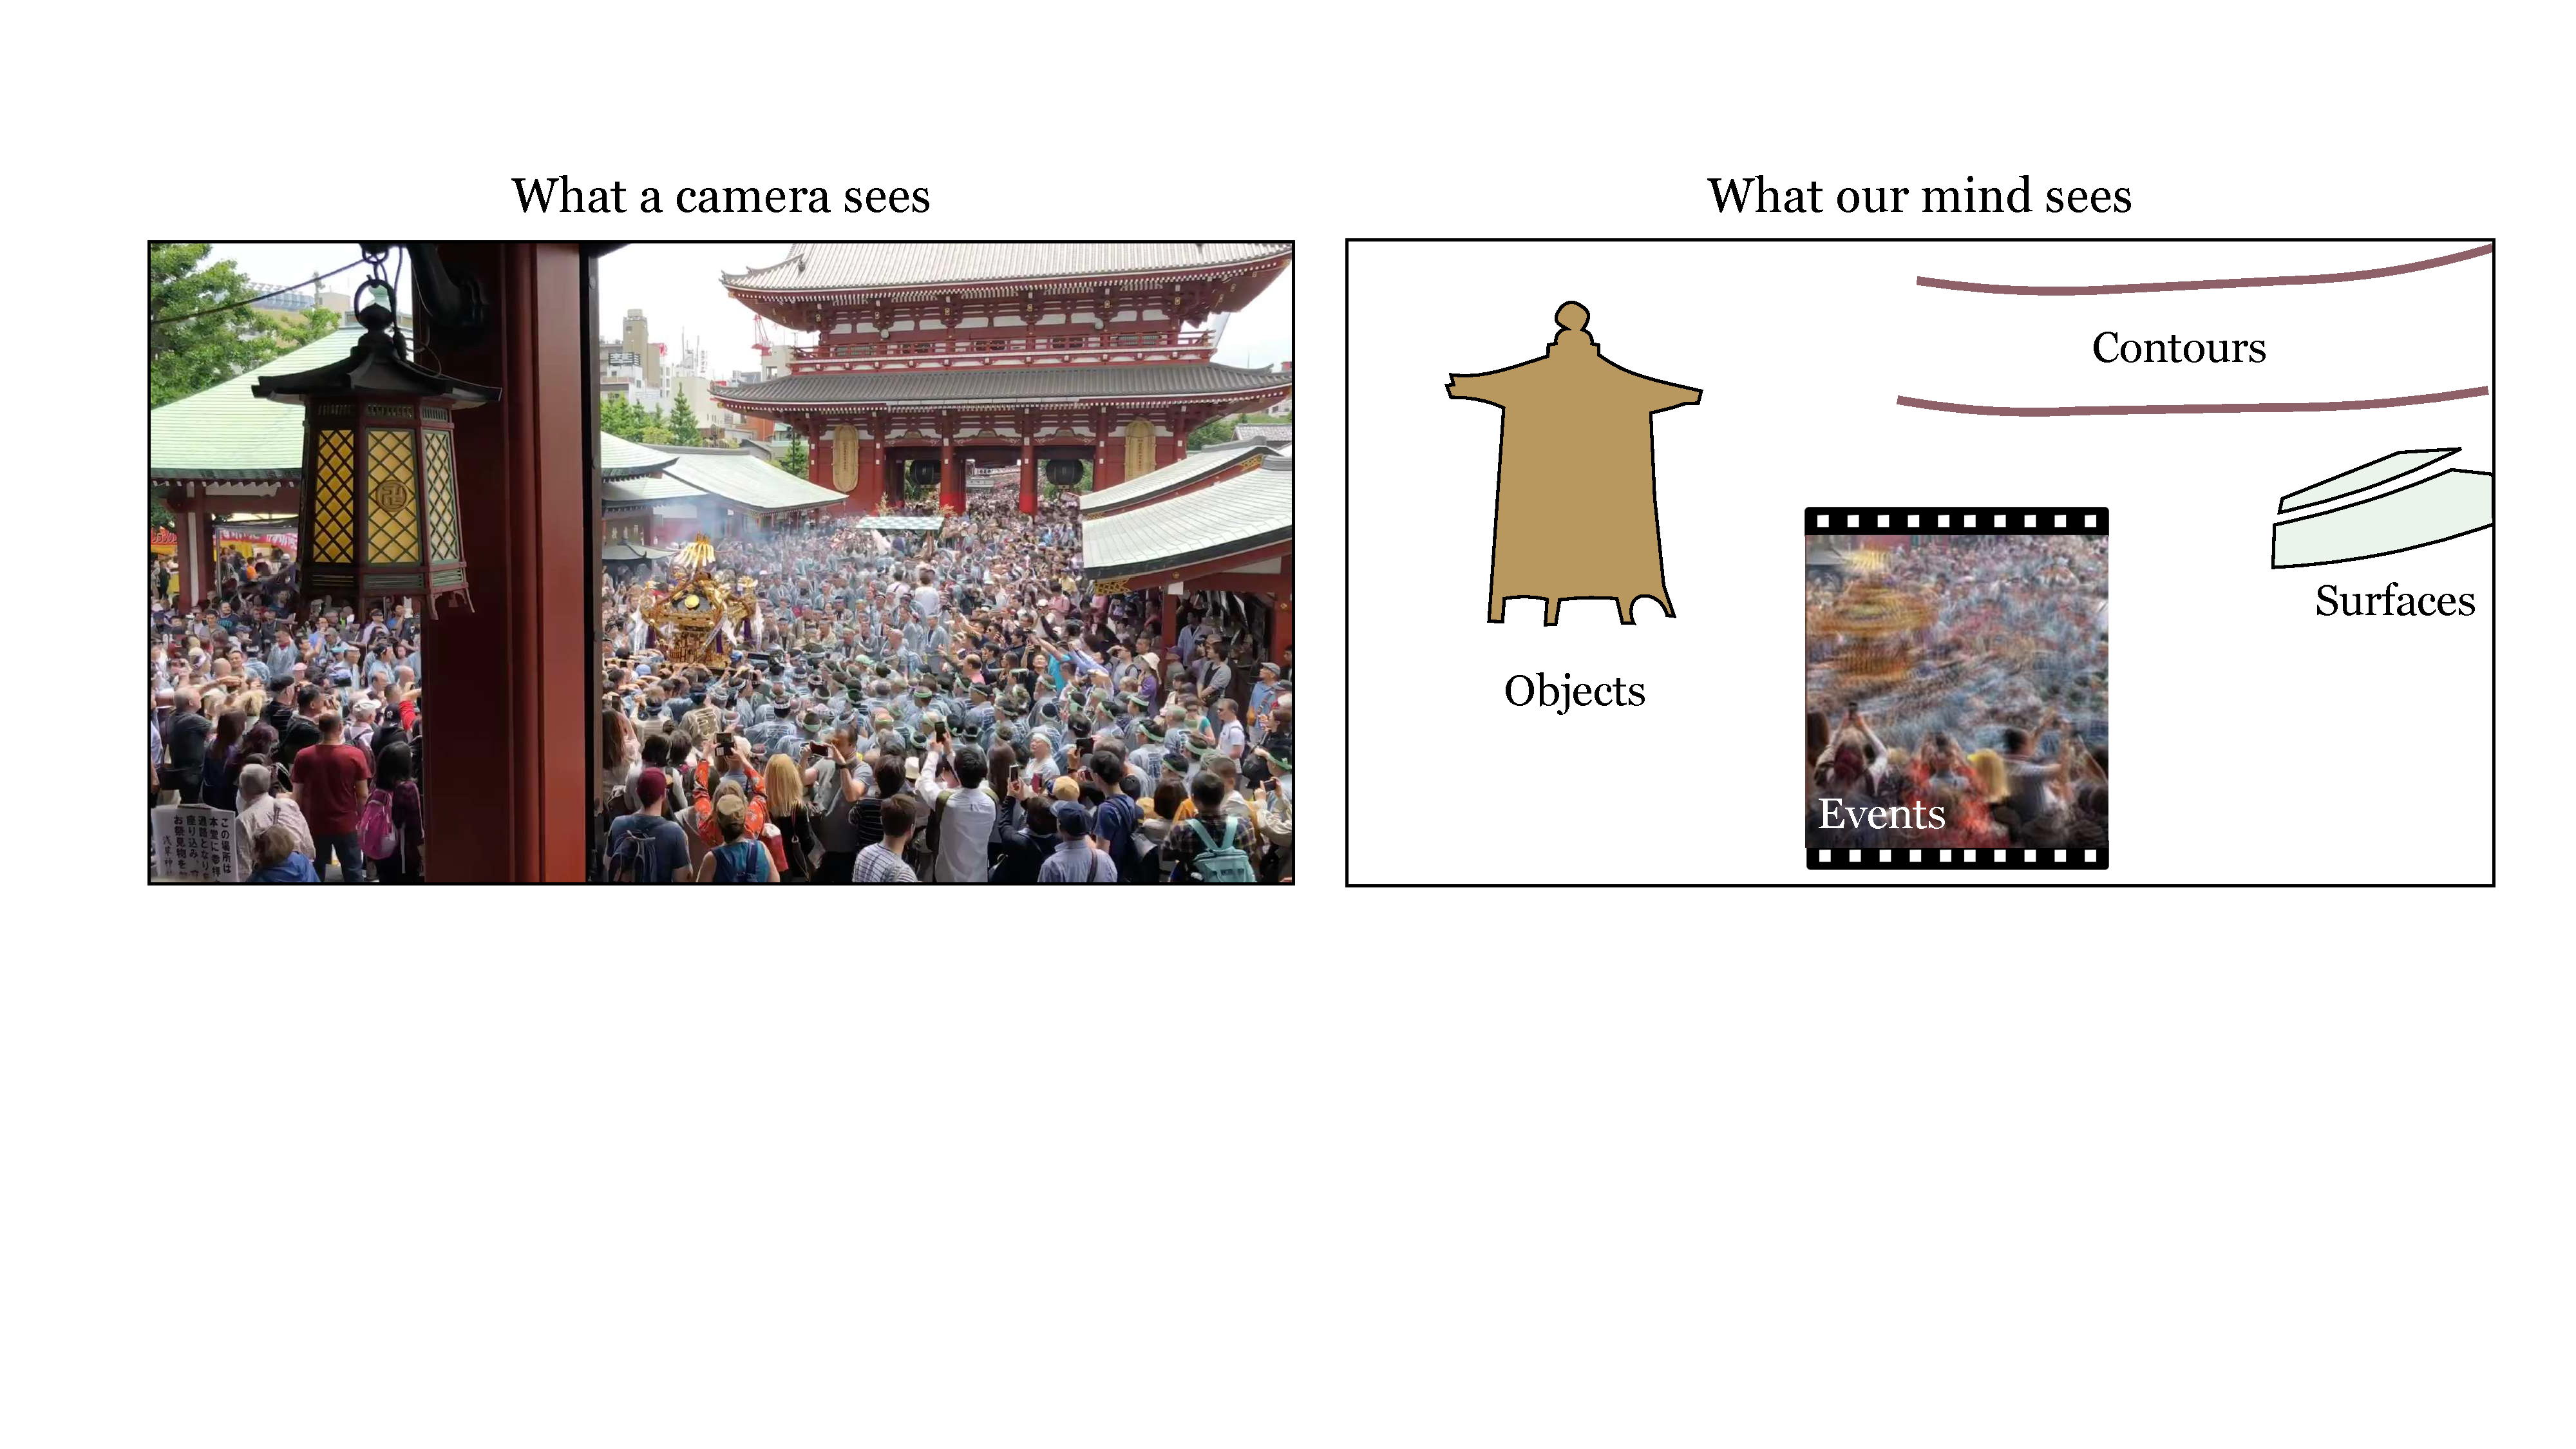
\includegraphics[width=1.0\linewidth]{./figures/perceptual_organization/perc_org_teaser.pdf}
    }
    \caption{A few kinds of perceptual organization in the human visual system.}
    \label{fig:perceptual_organization:perc_org_teaser}
\end{figure}

What a camera sees is the raw RGB pixel values of the photo. But what your mind sees is rather different. You see contours and surfaces, objects and events.

Many of these perceptual structures can be thought of as \textit{groups of primitive elements}: a contour is a group of points that form a line, an object is a group of parts that form a cohesive whole, and so on. Because of this, understanding how humans, and machines, can identify meaningful perceptual groups has been a longstanding area of interest in both human and computer vision~\cite{Palmer1999}. %The study of \textbf{perceptual organization} therefore largely revolves around the study of \textbf{perceptual grouping}.
\marginnote{The content of this chapter can also go under the name \index{Perceptual organization}\textbf{perceptual organization}, which is the study of how our vision system organizes the pixels into more abstracted structures, such as perceptual groups. The Gestalt psychologists were some of the first to study this problem~\cite{Koffka1935}.}[-4.4cm]

%\section{Principles of Grouping}
This leads us to a central question: which primitives should be grouped? We will examine a few answers below, including the idea that primitives should be grouped based on \textit{similarity} or based on \textit{association}. We will also look at how natural groups can emerge as a byproduct of a downstream purpose.

\section{Why Group?}
Grouping is a special case of representation learning, and the reasons to group are the same as the reasons to do representation learning: groups are a good substrate for downstream analysis and processing. To get an intuition for why this is, consider how you might describe the scene around you. Go ahead and write down what you see. If you are in a cafe, you might write, ``I'm sitting at a table with my laptop in front of me. A latte is next to the laptop; the foam and coffee are swirling into a spiral.''
%\marginnote{You might find it odd to refer to grouping as \textit{learning}. Shouldn't we say ... Grouping is learning. Learning to group is meta-learning.}

Now let's look at each of these words. Some refer to objects (e.g., ``table'', ``laptop'', ``latte''). Others refer to spatial relationships (``in front'', ``next to''), and still others refer to shapes (``spiral'') and events (``swirling''). These kinds of structures—objects, relationships, shapes, events—are the elements of perceptual organization, and you can think of perceptual organization as being a lot like describing an image in text. One of the hottest current trends in computer vision is to map images to text, then use the tools of natural language processing to reason about the image content. In this way text is treated as a powerful image representation, and indeed it has become clear that this kind of image representation—symbolic, discrete, semantic—can be exceedingly effective~\cite{alayrac2022flamingo,wu2023visual,gupta2023visual,suris2023vipergpt}.

Perceptual organization is all about trying to get similarly powerful representations, but doing so via bottom-up grouping rules, rather than by mimicking human language. In other words, perceptual organization is about \textit{discovering} language-like structures in the first place, from unsupervised principles rather than from human-language supervision. Why do we have the words we have, where did they come from? What exactly is an \textit{object}? This chapter may start to provide some answers.

Although the analogy to text makes clear why perceptual organization is important, perceptual groups can also go beyond the limits of language. Some structures we see are hard to name but still clearly represent a coherent group in our heads. Consider, for example, the image in \fig{\ref{fig:perceptual_organization:perc_org_nonsemantic_example}} below.
\begin{figure}[h]
    \centerline{
        
\includegraphics[width=0.35\linewidth]{./figures/perceptual_organization/perc_org_nonsemantic_example.pdf}
    }
    \caption{How many objects do you see?}
    \label{fig:perceptual_organization:perc_org_nonsemantic_example}
\end{figure}

There are clearly two separate objects, but we don't have names for them.
%One of the hottest current topics is to map images to text, then use the tools of natural language processing to reason about the image content. In this way text is treated as a powerful image representation. The elements of text -- names for objects and events, names for relationships between entities, etc -- are essentially the same as the classical elements of perceptual organization -- objects, events, relationships. One way to think about perceptual organization is therefore as mapping images to text strings like ``an X next to a Y in front of a Z." X, Y, and Z are perceptual groups (perhaps objects) which are further organized by spatial and layering relationships. The main differences between the study of perceptual organization and the study of image-to-text are 1) perceptual structures do not \textit{only} correspond to entities for which we have words; they could go beyond the limitations of our finite vocabulary, and 2) perceptual organization focuses on discovering these structures from unlabeled data, whereas image-to-text systems are typically supervised to simply imitate human-generated data (e.g., image captions on the internet).
%
%Before we start, what, mathematically, do we mean by ``perceptual group"? Generally this refers to a variable that selectively responds only to particular conjunctions of primitives. For example, this variable could take on a value of 1 to indicate the presence of a group and 0 otherwise.
%
% -- New outline for segmentation part --
% * Segmentation is mathematically a clustering problem
% * So let's try k-means, which you saw in rep learning chapter
% * It is okay but: 1) sensitive to k, 2) sensitive to init, 3) can split connected components (gradient example), 4) doesn't work on naive features (color, texture?)
% * Other methods have been developed to get around some of the issues with k-means: linkage based methods get around #3, some things like mean shift select k
% * But the main thing is you just need better features / better affinity measure
% * So we could learn these unsupervised in a way designed for segmentation
% * Or just let them emerge from any representation learning method or downstream task
%
% -- show 2D ab plot of pixel colors in an image
% -- show kmeans on this
% -- show MRF on this (continuity principle)
% -- show same but with better affinities
% -- semantic segmentation: reduce the problem to recognizing familiar objects
% -- emergent segmentation: segmentation must be useful since neural nets learn to do it in their hidden layers
The next sections will cover a few different kinds of perceptual groups that are important in vision.

\section{Segments}

\index{Segmentation}\textbf{Segmentation} is the problem of partitioning an image into regions that represent different coherent entities. There is no single definition of what is a coherent entity and it will vary depending on the task; a segment could correspond to a nameable object, or a image region made of a single material, or a physically distinct piece of geometry (see \fig{\ref{fig:perceptual_organization:ambiguous_segmentation_example}}).

Segmentation can be framed as a clustering problem: assign each pixel in an image to one of $k$ clusters. We will explore two approaches to solving this clustering problem: (1) assign similar pixels to the same cluster, (2) assign two pixels to the same cluster if there is no boundary between them. We will start with the first.

\begin{figure}[h!]
    \centerline{
        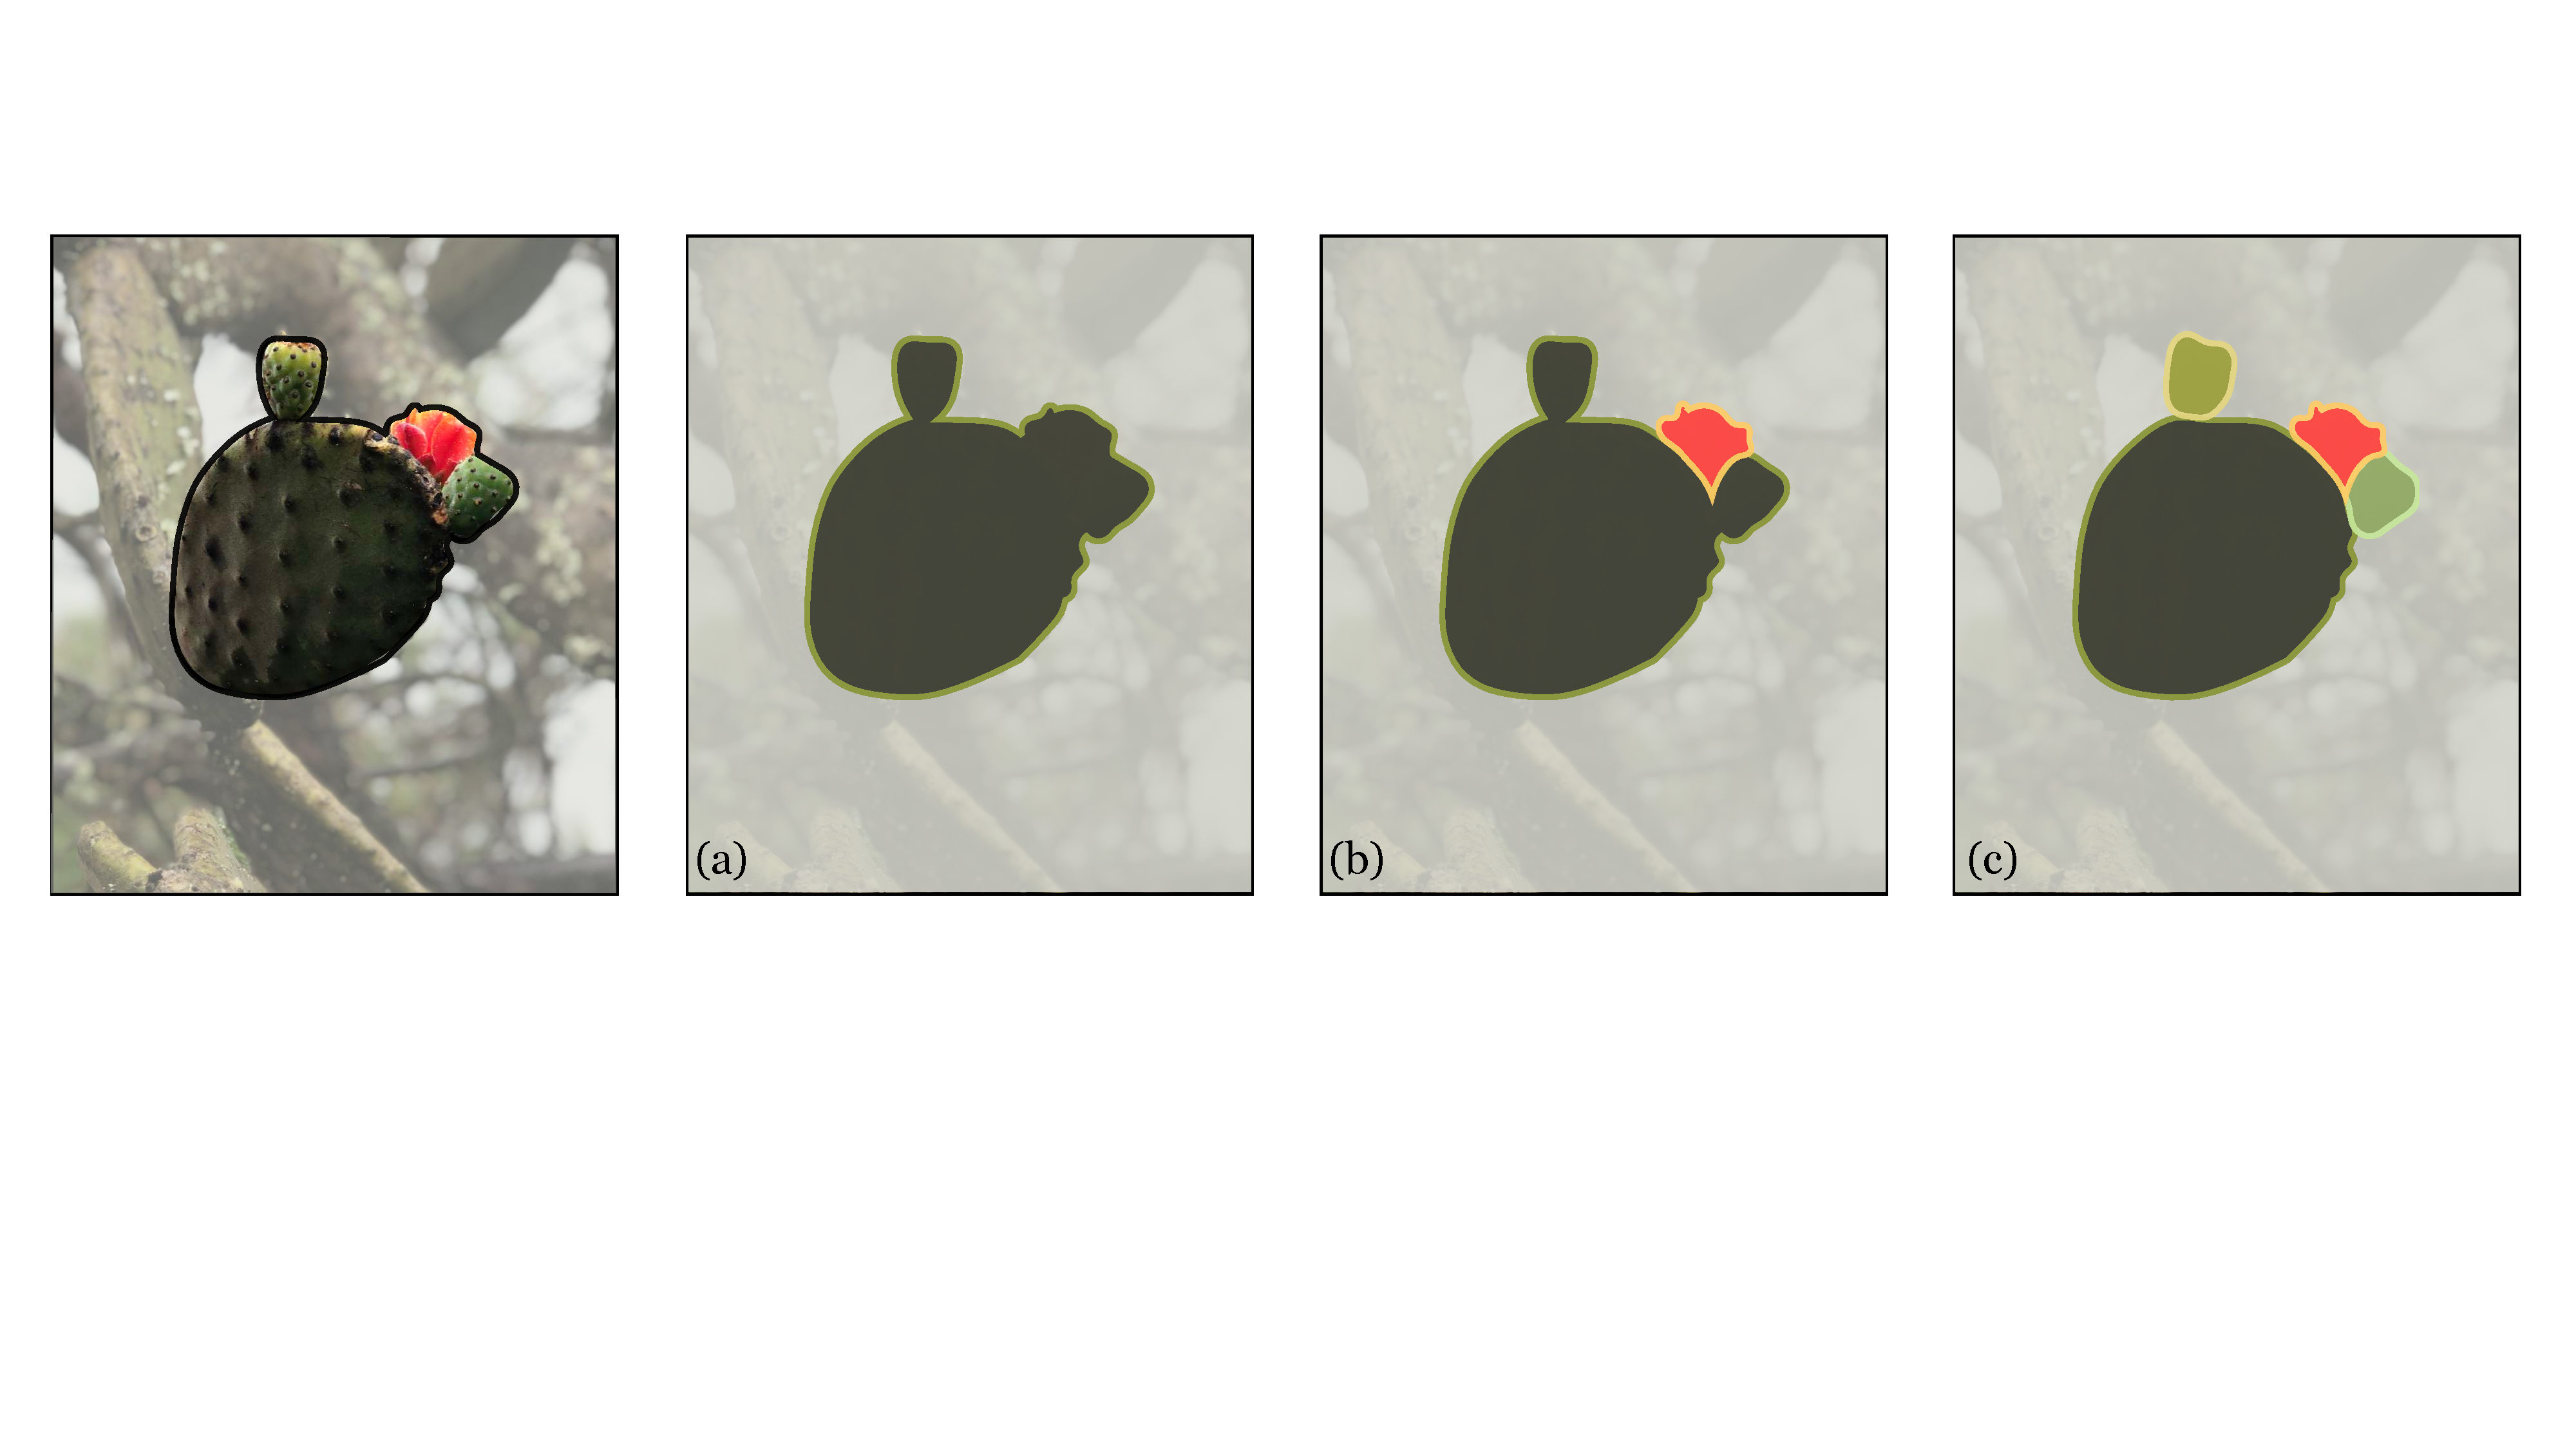
\includegraphics[width=1.0\linewidth]{./figures/perceptual_organization/ambiguous_segmentation_example.pdf}
    }
    \caption{There are multiple ways you might segment any given image, and each way will highlight different world properties. This cactus branch could be viewed as (a) a single segment (the ``branch''), (b) two segments (the ``leaf" and the ``flower''), or (c) four segments (the main ``leaf,'' two ``buds,'' and the ``flower'').}
    \label{fig:perceptual_organization:ambiguous_segmentation_example}
\end{figure}
\vspace{-0.4cm}

\subsection{$K$-Means Segmentation}
\index{K-means segmentation}
$K$-means, which we covered in \chap{\ref{chapter:representation_learning}}, is one of the simplest and most useful clustering algorithms, so let's try it for segmentation.

$K$-means operates on a data matrix of $N$ datapoints by $M$ features per datapoint. Our first task is to convert the segmentation problem to that format. The simplest thing to do is let each pixel be a datapoint and the pixel's color be its feature vector. For ease of visualization, we will use the $ab$ color value as the two-dimensional (2D) feature per pixel. An image represented this way can be plotted as a scatter plot and you can think of it as samples from a distribution over $ab$ colors, as shown in \fig{\ref{fig:perceptual_organization:scatter_ab_fruits2}}.
\vspace{-0.4cm}
\begin{figure}[h!]
    \centerline{
        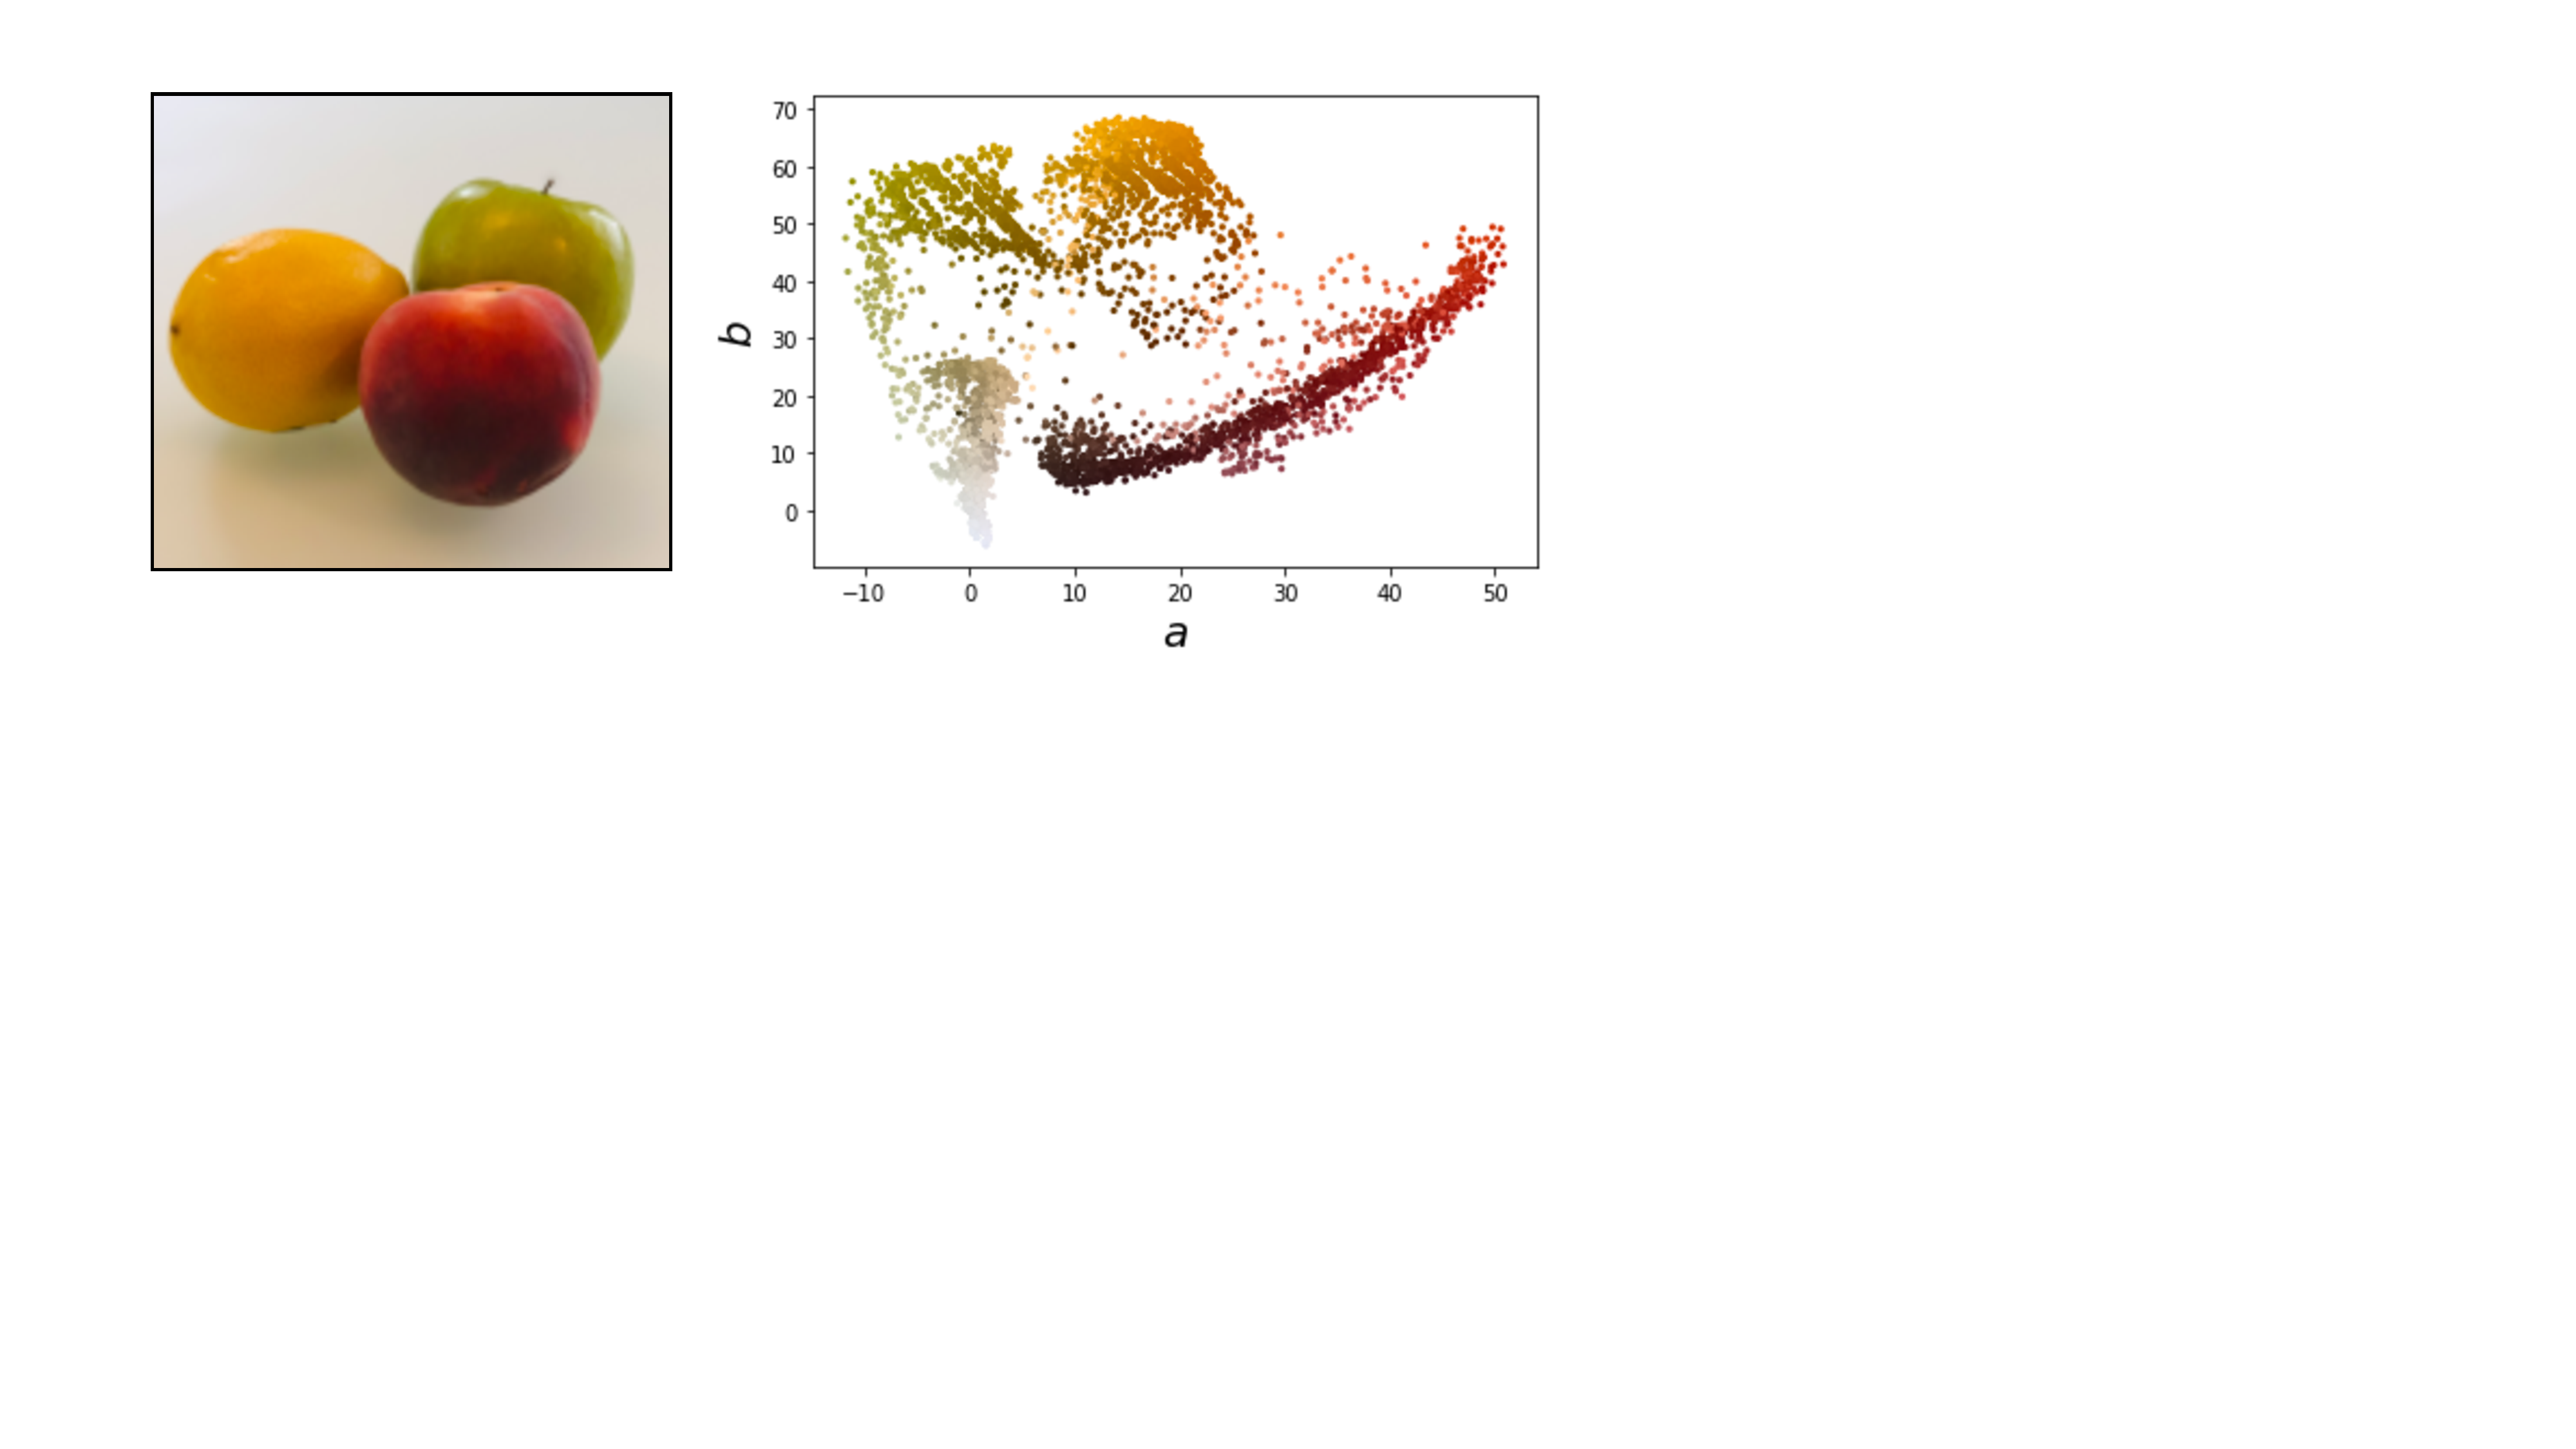
\includegraphics[width=0.75\linewidth]{./figures/perceptual_organization/scatter_ab_fruits2.pdf}
    }
    \caption{Different regions of coherent color in the image correspond to clusters in the scatter plot of all the $ab$-values of the image's pixels. In general, segmentation can be reduced to the problem of \textit{clustering pixels} in some feature space ($ab$-color in this example, but it can be any pixel-wise feature).}
    \label{fig:perceptual_organization:scatter_ab_fruits2}
\end{figure}
\vspace{-0.4cm}


$K$-means tries to find clusters in this scatter plot (and, if you prefer a probabilistic interpretation, it can be thought of as fitting a mixture of Gaussians to the datapoints, which aims to approximate the distribution from which these pixels were sampled). We can segment via $k$-means by simply assigning each pixel to the cluster assignment of its color value. Below we color each pixel in each cluster by the mean color of all pixels assigned to that cluster (\fig{\ref{fig:perceptual_organization:kmeans_ab_fruits2}}).
\vspace{-0.4cm}
\begin{figure}[h!]
    \centerline{
        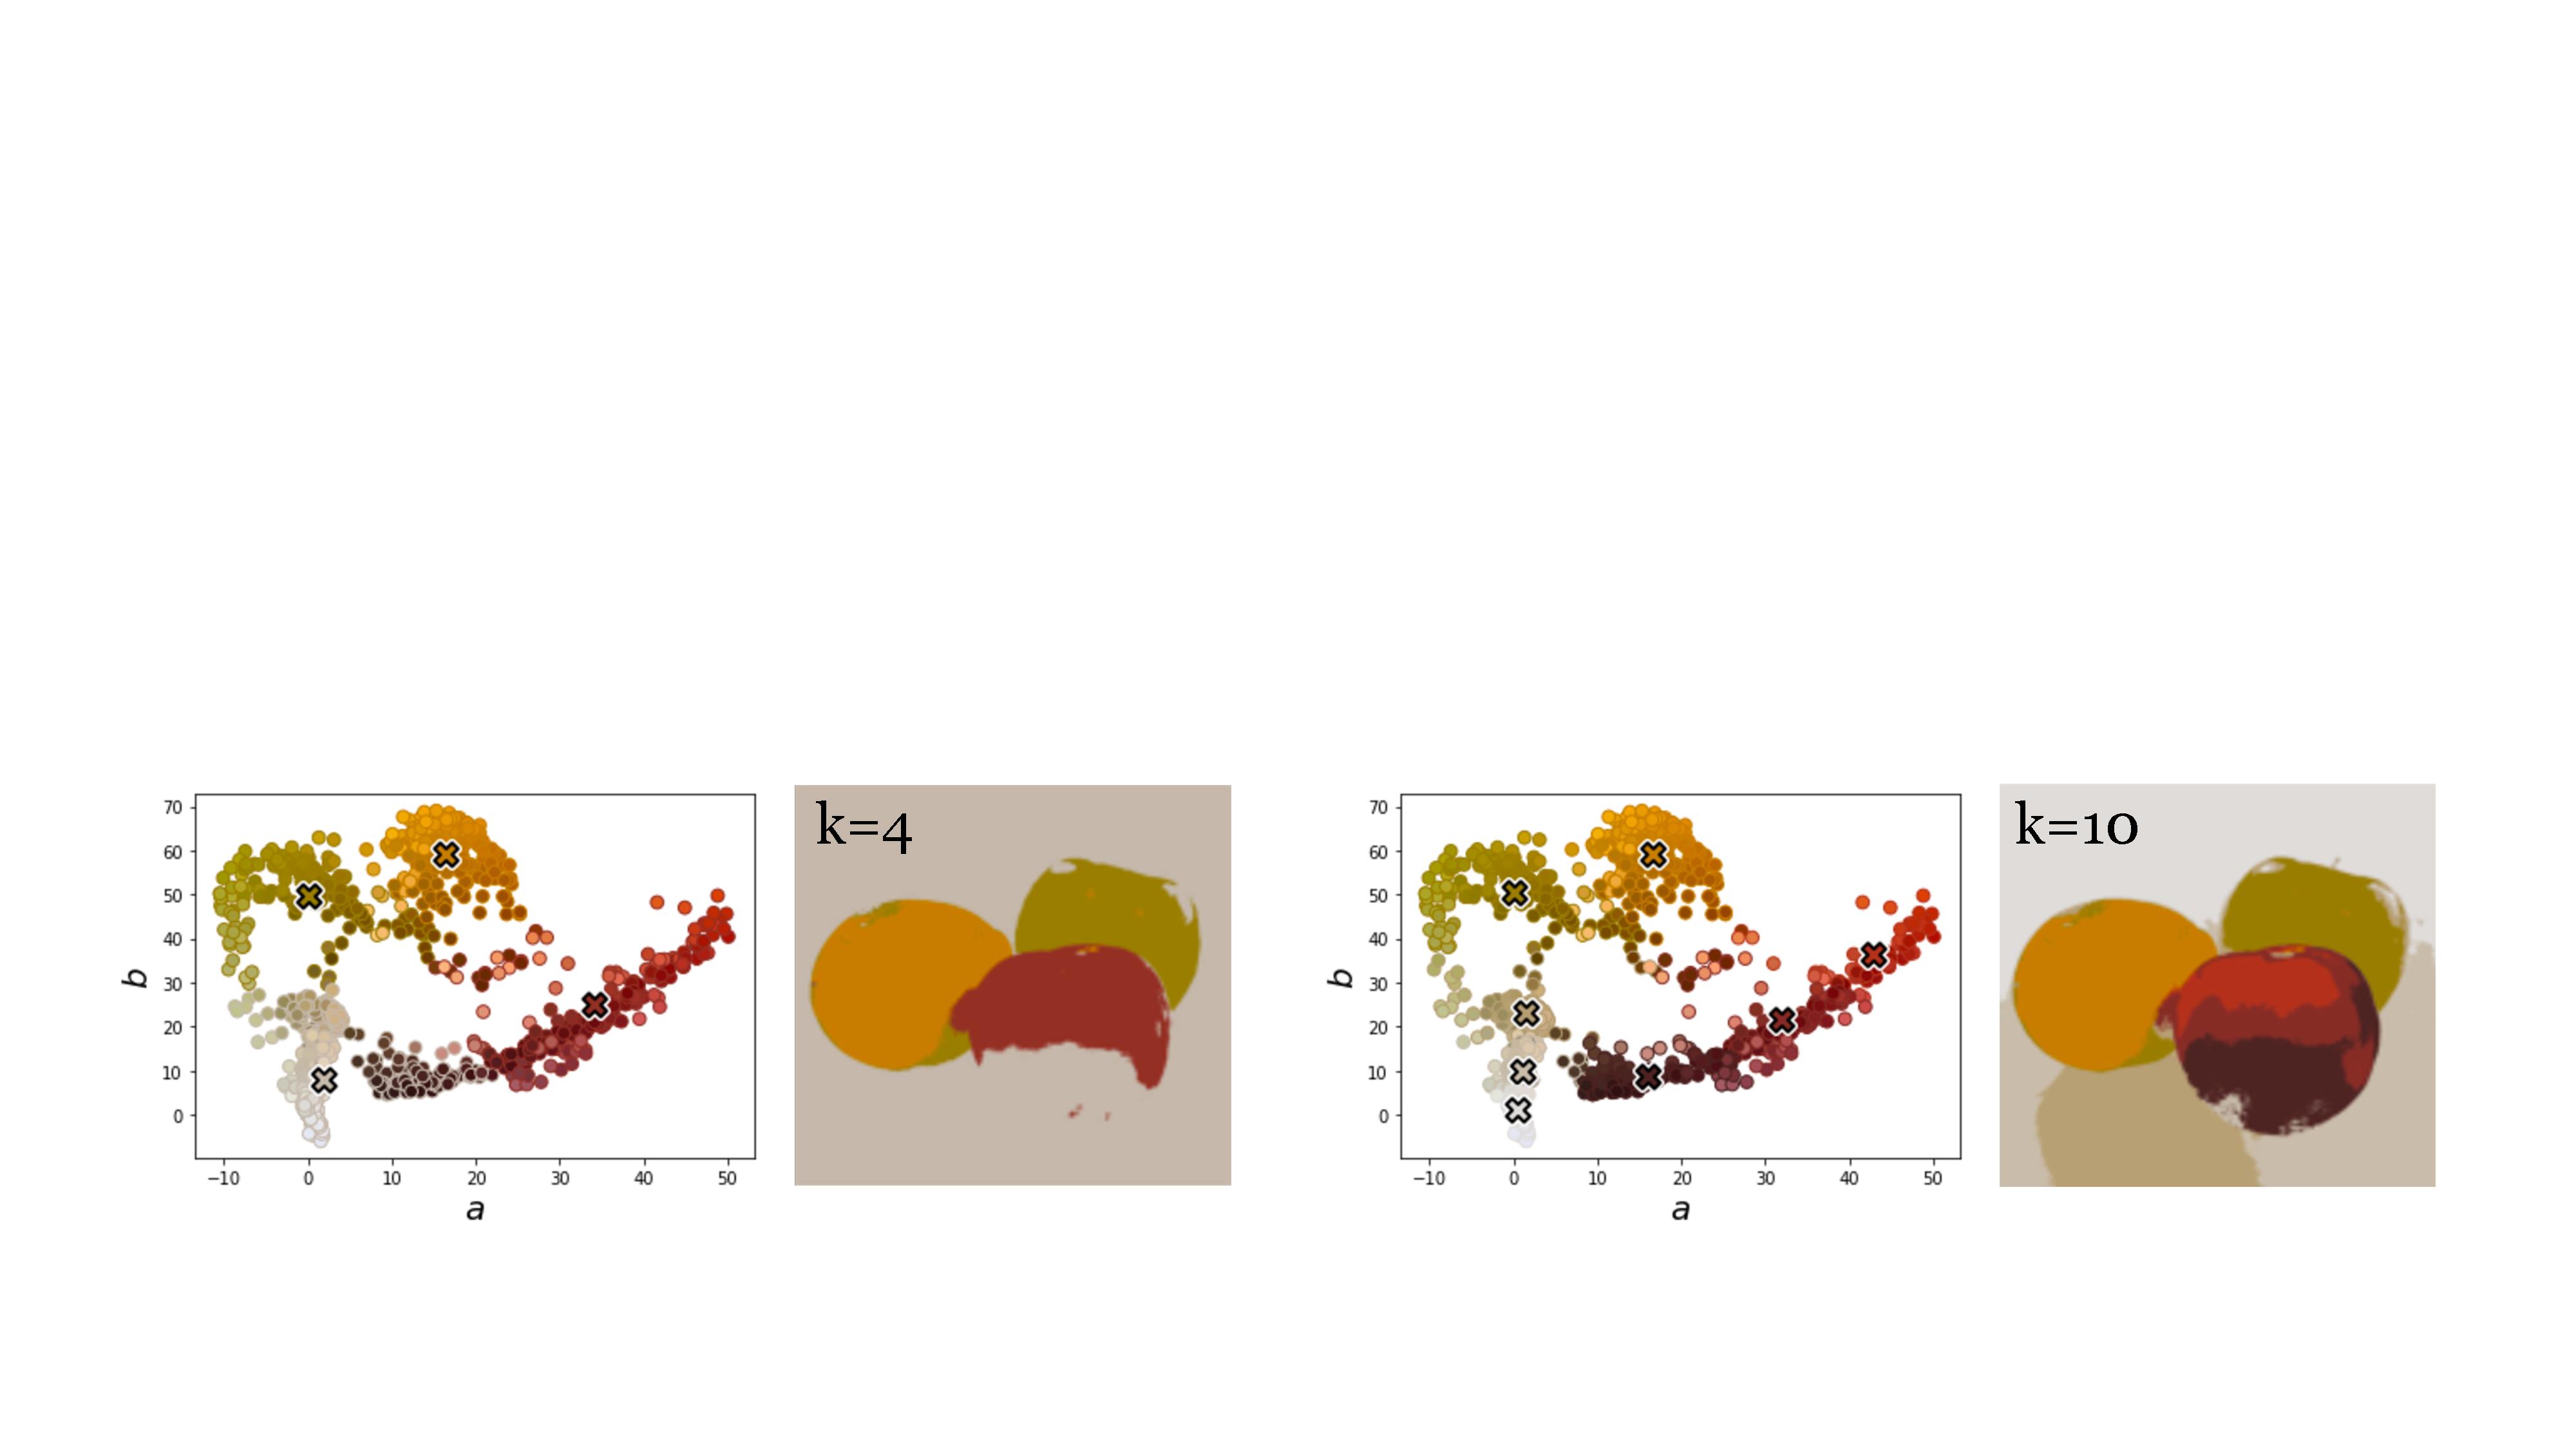
\includegraphics[width=1.0\linewidth]{./figures/perceptual_organization/kmeans_ab_fruits2.pdf}
    }
    \caption{$K$-means segmentation on the fruits example.}
    \label{fig:perceptual_organization:kmeans_ab_fruits2}
\end{figure}

Naturally, $k$-means on $ab$-values finds segments that correspond to regions of roughly a constant color. This simple approach can be surprisingly effective. notice how it segments a zebra from the background in \fig{\ref{fig:perceptual_organization:kmeans_ab_zebra_and_beach}} (because the black and white stripes have roughly the same $ab$-values). However, it fails to group more complex patterns that are not defined by color similarity, as in the beach photo in \fig{\ref{fig:perceptual_organization:kmeans_ab_zebra_and_beach}}.
\begin{figure}[h!]
    \centerline{
        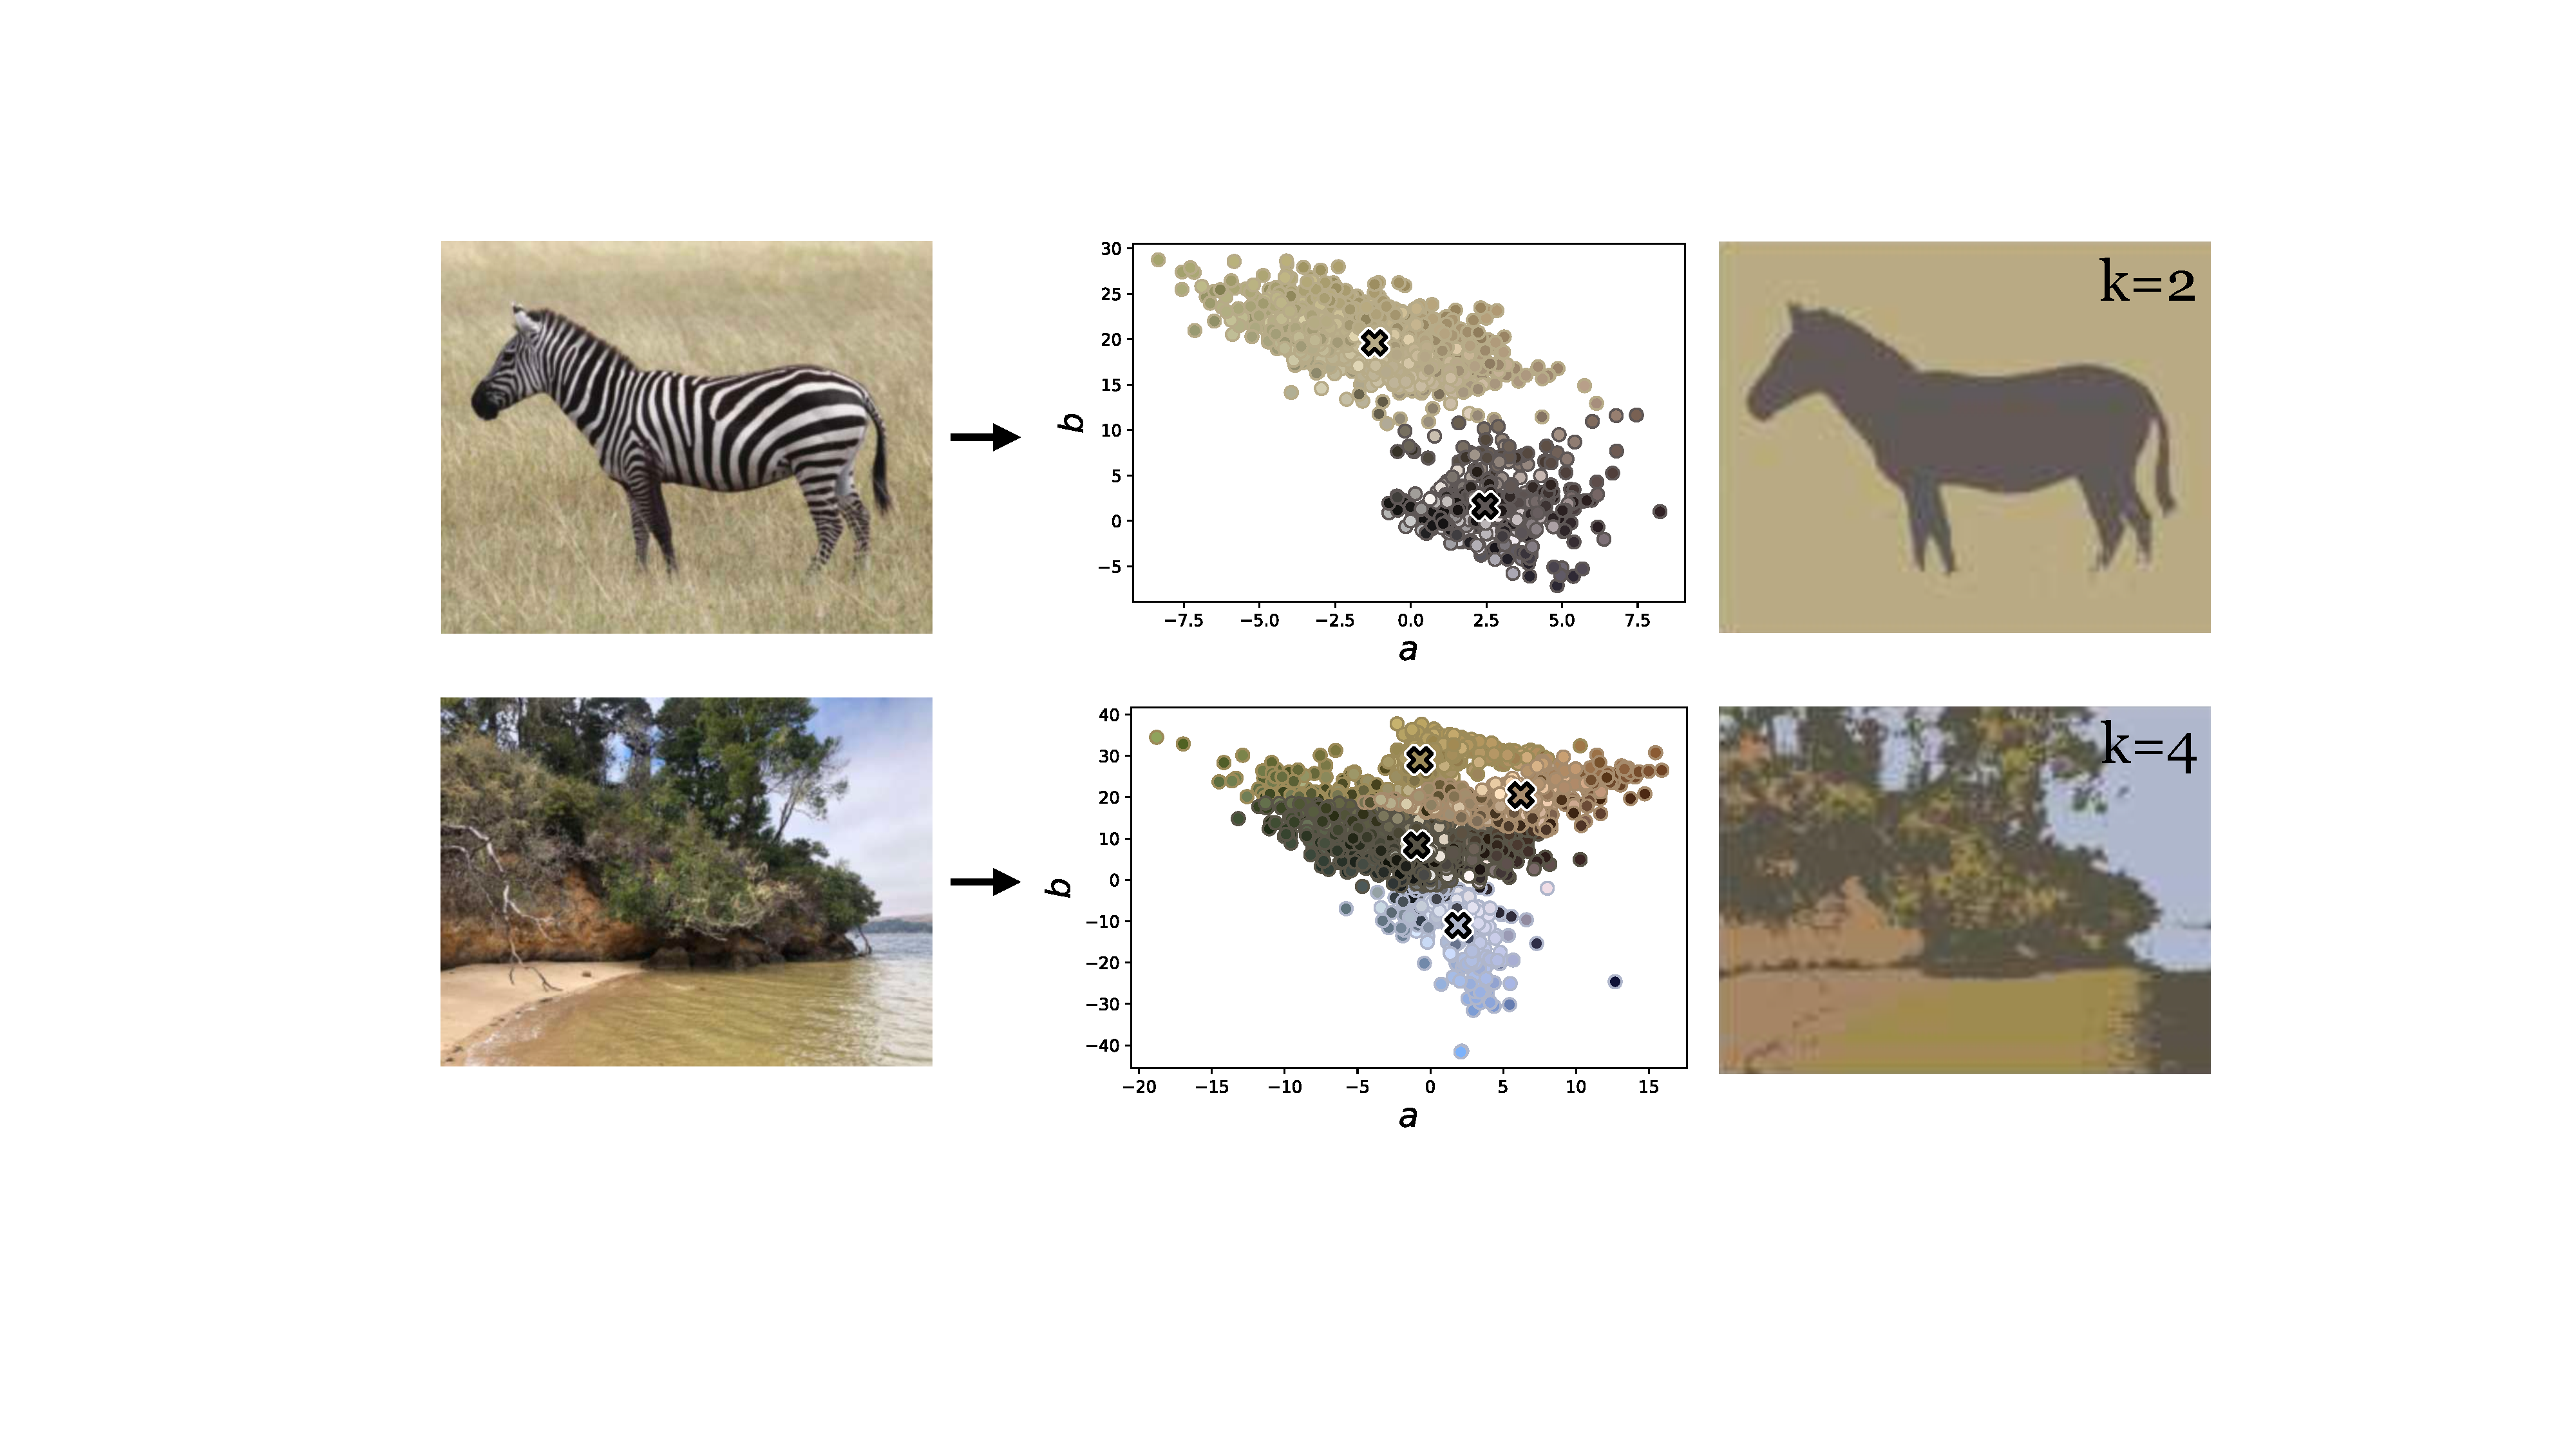
\includegraphics[width=1.0\linewidth]{./figures/perceptual_organization/kmeans_ab_zebra_and_beach.pdf}
    }
    \caption{(top row): $k$-means segmentation succeeds on a seemingly hard image. \textit{Photo source}: Fredo Durand. (bottom row): $k$-means fails on an image that, to our eye, looks no more complex.}
    \label{fig:perceptual_organization:kmeans_ab_zebra_and_beach}
\end{figure}
\vspace{-0.4cm}

\subsection{Affinity-Based Segmentation}\label{sec:perceptual_organization:affinity_based_segmentation}
\index{Affinity-based segmentation}
Other clustering methods are based on the idea of \textbf{affinity}, where we try to model a distance metric (the affinity) that tells us whether two items should be grouped. The distance metric usually measures how similar two patterns are, or how likely they are to be part of the same object.

For example, a simple affinity function over pixel pairs could just be the Euclidean distance between the color values of the two pixels. There are numerous ways we could use such an affinity to group pixels into segments, all of which share the general idea that pixels with high affinity should belong to the same group and pixels with low affinity should belong to two different groups. Methods that use this idea include those based on graph cuts~\cite{shi2000normalized}, spectral clustering~\cite{arbelaez2010contour}, and Markov random field (MRF)-based clustering (\chap{\ref{chapter:probabilistic_graphical_models}}).

We do not have time to cover all these methods and in fact they are no longer commonly used. Instead we will focus on a method you have seen earlier in the book that actually is in common use: contrastive learning (which was covered in \sect{\ref{sec:representation_learning:contrastive_learning}}). Contrastive learning is a perfect fit for affinity-based segmentation because contrastive methods learn from similarities (positive pairs) and differences (negative pairs), and this is what an affinity metric gives us! Contrastive methods learn an embedding in which datapoints with high affinity are nearby and datapoints with low affinity are far apart. Once we have such an embedding, clustering is easy in the embedding space, and pretty much any off-the-shelf clustering algorithm will work; for simplicity, we will stick with $k$-means in this book.\marginnote{In this book we only present one way to do affinity-based clustering: first use affinities to supervise a embedding in which the data is nearly clustered, then read off the clusters using a simple quantization method like $k$-means. There are many other affinity-based methods but this simple method often works well.}[-2.5cm]

If we define affinities in terms of color distance, then there's no point in \textit{learning} such an embedding, because the raw colors themselves are already a great embedding under that notion of affinity. Affinity-based clustering only really becomes interesting when we have nontrivial affinities to model; for example, they could be given by human judgments about which pixels should go together in natural images.

Because human supervision is expensive and limiting, a popular alternative is to use self-supervised affinity measures, just like we saw in self-supervised contrastive learning. Popular contrastive learning methods like SimCLR~\cite{chen2020simple}, MoCo~\cite{he2020momentum}, and DINO~\cite{caron2021emerging}, train a mapping from image patches to embedding vectors such that two patches that come from the same image embed near each other and patches from different images embed far apart. We can run these methods \textit{densely} (in a sliding window fashion) across a single image to create a feature map of size $C \times N \times M$, where $N$ and $M$ are the spatial dimensions of the feature map and $C$ is the dimensionality of the embedding vectors. This creates a new image where each pixel has a value (the embedding vector) that is similar to other pixels that the model thinks would be likely to appear in the same scene. In effect, we have learned an affinity metric based on natural patch co-occurrences, then used that affinity metric to obtain a feature map that reveals the coherent regions of an image. If we apply $k$-means to the pixels in this feature map, we can obtain an effective segmentation. This entire pipeline is shown in \fig{\ref{fig:perceptual_organization:kmeans_dino}}, using DINO~\cite{caron2021emerging} as the particular contrastive embedding.

%In fact, we have already seen on method that uses color affinities to arrive at segments: the k-means example from the preceding Section! In k-means, the objective function penalizes the distance between each cluster's center and it's assigned datapoints. In our example that was the color affinity between 

\begin{figure}[t]
    \centerline{
        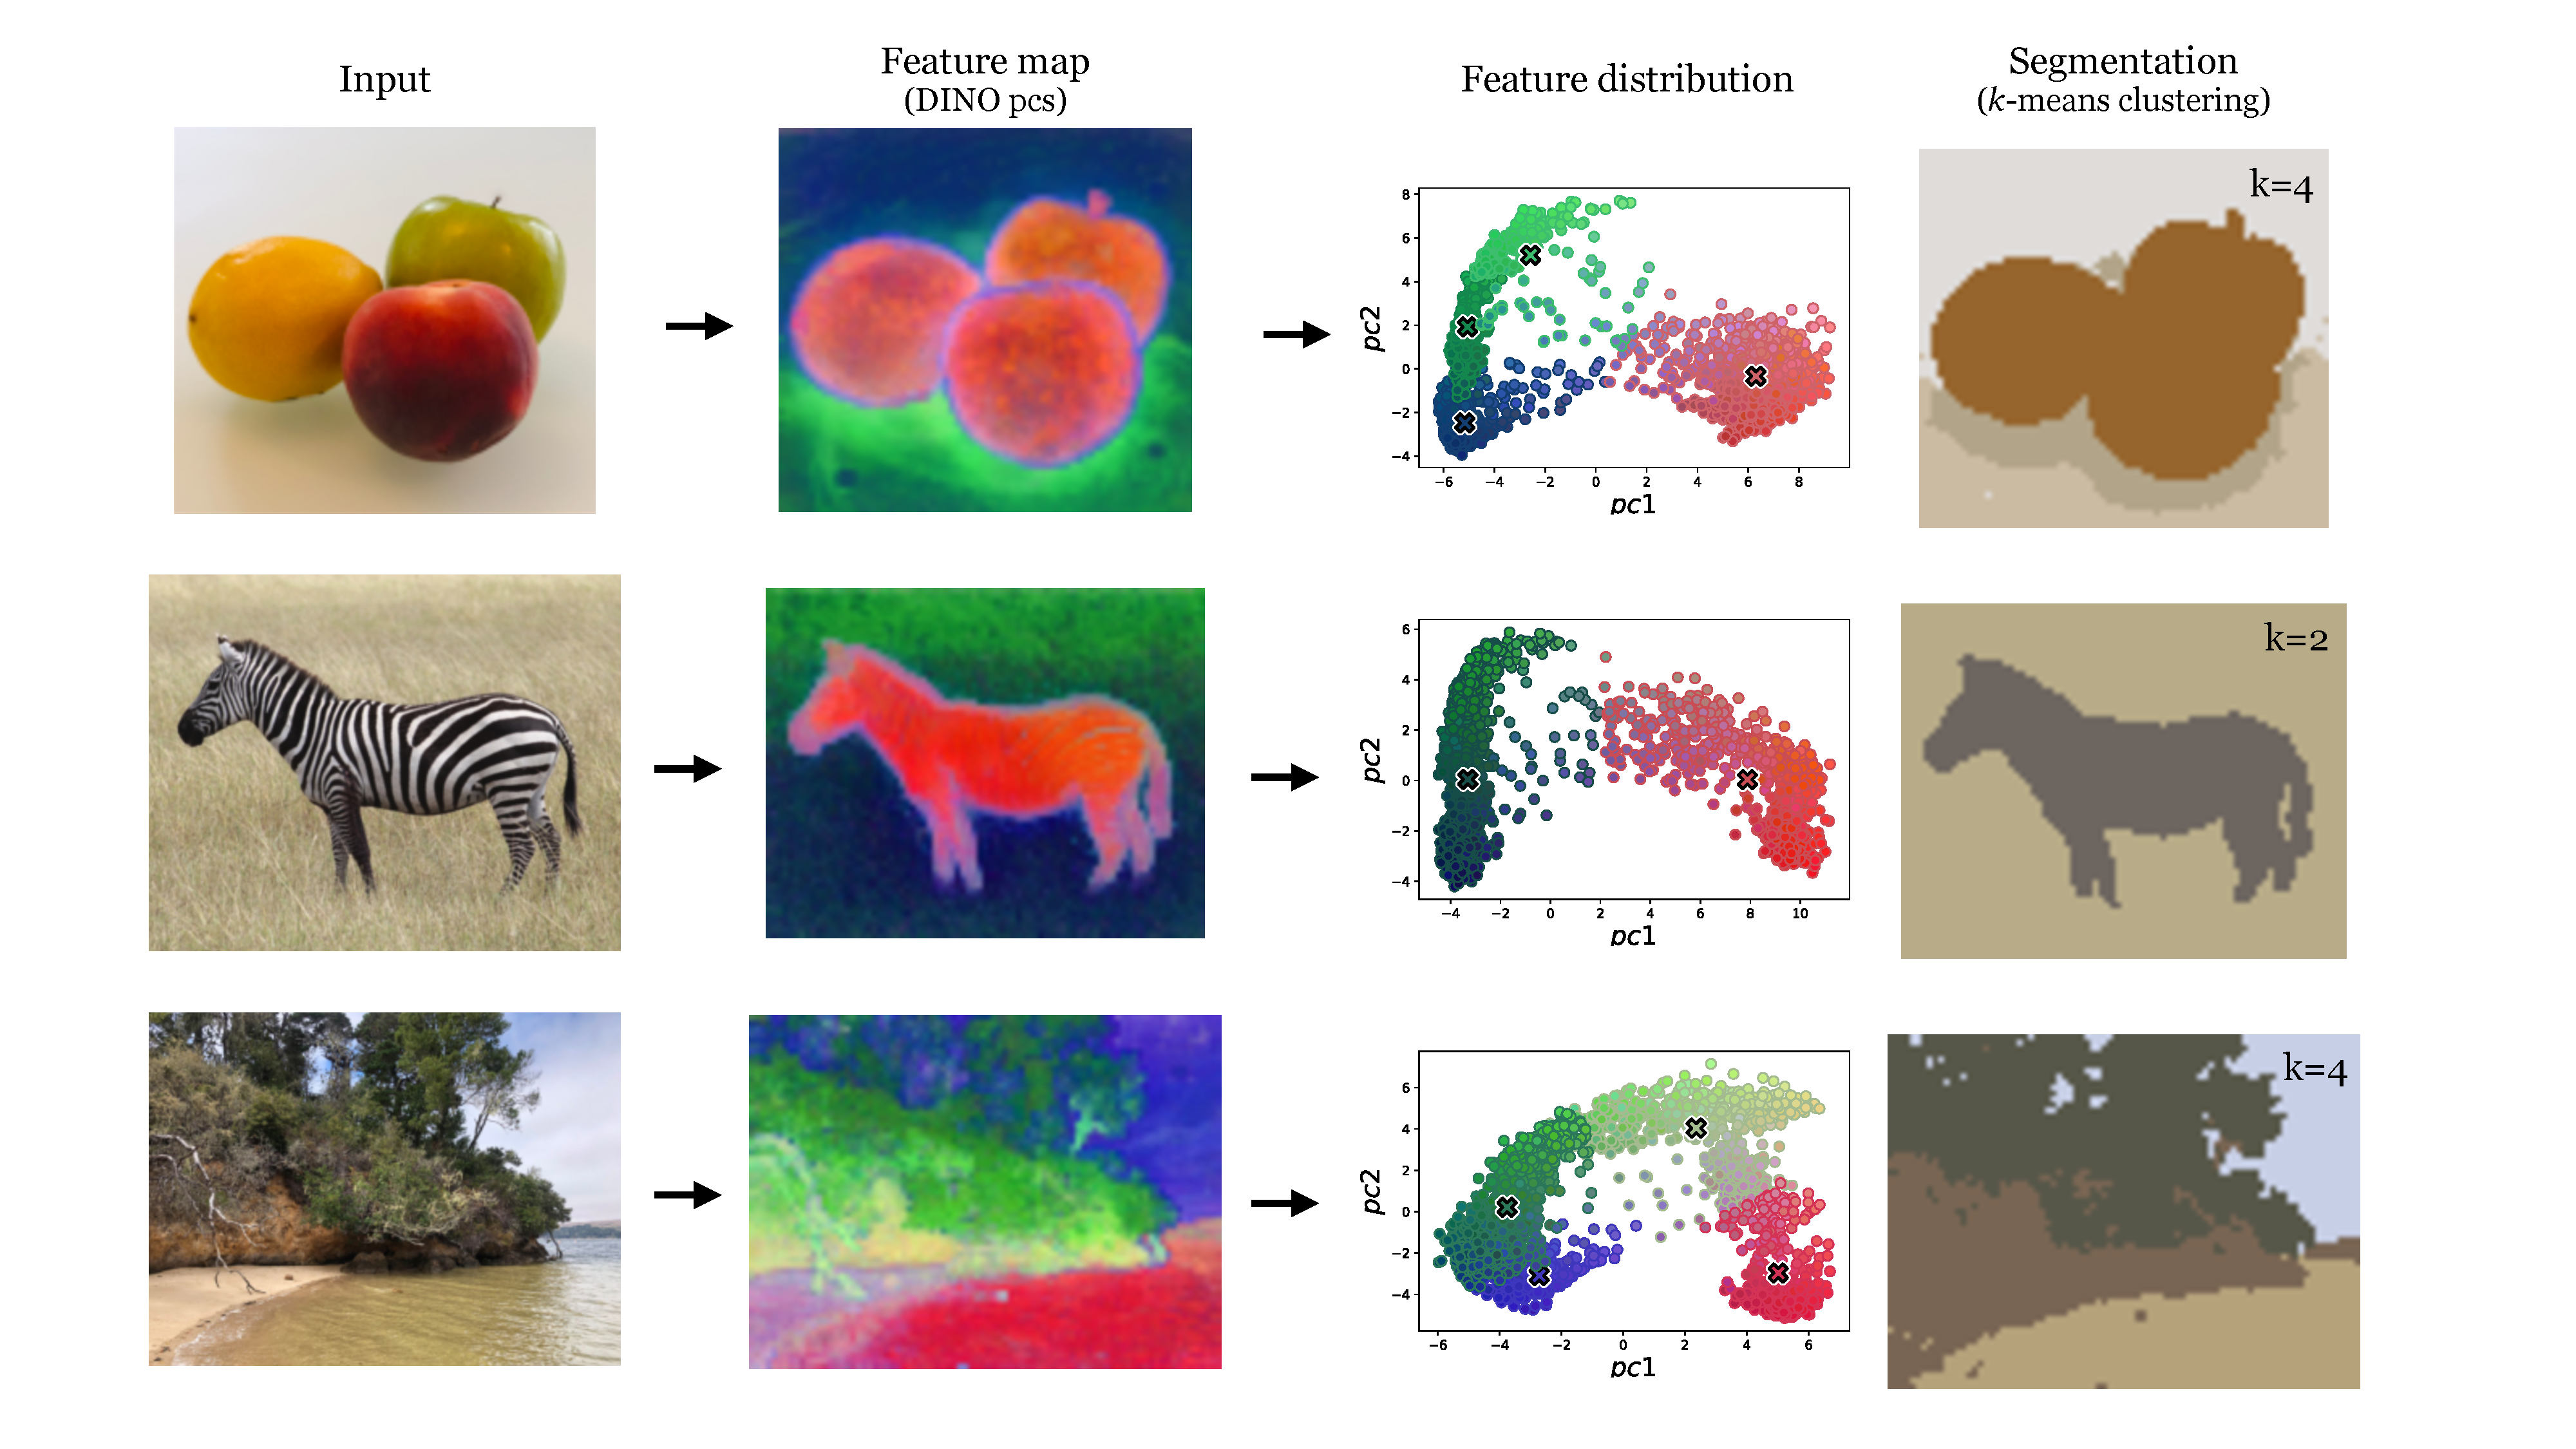
\includegraphics[width=1.0\linewidth]{./figures/perceptual_organization/kmeans_dino.pdf}
    }
    \caption{Image segmentation using $k$-means over DINO~\cite{caron2021emerging} features.}
    \label{fig:perceptual_organization:kmeans_dino}
\end{figure}

\section{Edges, Boundaries, and Contours}
A complementary problem to segmentation is boundary detection, because a partitioning of an image can be represented either by partition assignments (segments) or by the boundaries between partitions. Many vision algorithms organize images into different kinds of boundaries between perceptual structures. Early vision algorithms focused on \index{Edge detection}\textbf{edge detection}, where the idea was that the edges in an image should form a good, compact representation of the image's content, because edges are relatively sparse, and they are stable with respect to nuisances like noise and lighting. Subsequent work identified connections between different kinds of edge structure and scene geometry; for example, an edge that represents an occluding contour indicates that there is a depth discontinuity at that location in the scene.

\Chap{\ref{chapter:simplesystem}} described some simple edge detectors and showed their use in reconstructing scene geometry. \Chap{\ref{chapter:3D_single_view}} covers more recent approaches to inferring three-dimensional (3D) scene structure, which have largely superseded the methods that explicitly reasoned about edges.

Line drawings are another way of representing the edge structure in an image, and they seem to be of high interest to humans. This suggests that there may be something useful about representing images in terms of their edge structure. Although there is an active line of research in computer graphics on modeling line drawings, this work has not yet paid off in vision, and it remains unclear whether or not line drawings will one day prove as compelling to visually intelligent machines as they do to us humans.


\section{Layers}
If you have ever seen an early Disney cartoon (e.g., Snow White), you may have noticed a compelling illusion of depth created by parallax between different layers of the animated scene.
\marginnote{
    An schematic of a multiplane camera from William E. Garity's 1940 patent for a ``Control Device for Animation.'' \\[6pt]
    \centerline{
        \setlength{\fboxsep}{0pt}
        \fbox{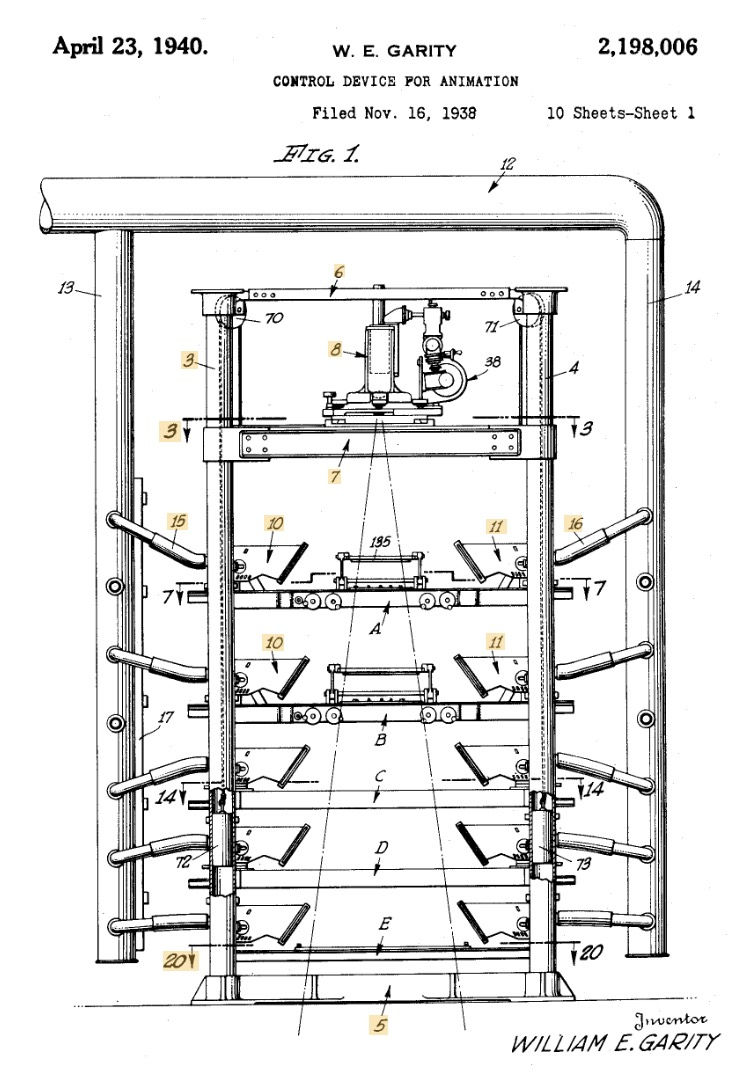
\includegraphics[width=.4\linewidth]{./figures/perceptual_organization/multiplane_patent.jpg}}
    }
}[-1.6cm]

Animators for these cartoons used a device called a multiplane camera, which worked as follows. A camera looked at a stack of glass planes. On each plane, the animators would draw a different \textbf{layer} of the scene. For example, on the back plane would be the sky, then there would be mountains on the next plane, then trees, and then the foreground characters. During filming the planes could be shifted back and forth to create parallax where the foreground planes move by more quickly than the planes further back.

This device works because it is a rough approximation to the actual 3D structure of the world. In computer vision, \index{Layer-based representations}\textbf{layer-based} representations like this have been popular as a way of capturing some aspects of depth without the expense of modeling a fully 3D world; sometimes layers and other related pseudo-3D representations are called \index{2.5D representations}\textbf{2.5D representations}.

Layers are not just an approximation to true depth, but also capture geometric structure that is \textit{not} well-represented by depth. Consider a pile of papers on your desk. The depth difference between one page and the next might only be a millimeter—too small to show up on standard depth sensing cameras. But the layer structure is obvious. Look back at \fig{\ref{fig:perceptual_organization:perc_org_nonsemantic_example}}: the depth \textit{order} is obvious even though you might have no idea how far apart these objects are in metric space. Layers capture \textbf{ordinal} structure and often this is the structure we care about; for example, if we want to pick up a piece of paper in our pile, the main thing that matters is if it is on top.

% \subsection{Ordinal depth}

% \subsection{Motion layers}

% \section{Objects}
% Objects can also be discovered via clustering.

\section{Emergent Groups}
It may seem like some of the topics in this chapter are out of fashion in modern computer vision. Edge detection and bottom-up segmentation are not the workhorses they once were. But this doesn't mean that perceptual organization is absent from current systems. These systems still see the world in terms of objects, contours, layers, and so forth, but those structures are emergent in their hidden layers rather than made explicit by human design. For example, in \fig{\ref{fig:representation_learning:obj_detectors_in_colorization}} we observed object detectors inside a neural net trained to do colorization.


\section{Concluding Remarks}
Perceptual organization aims to represent visual content in terms of modular and disentangled elements that make subsequent processing easier. In this way, perceptual organization shares the same goal as visual representation learning, although the former deals more with discrete structures whereas the latter has focused mostly on continuous representations. These two fields evolved somewhat separately, with perceptual organization having its roots in psychology and representation learning coming more from machine learning, but these days the end result is converging in the form of vision systems that see the world in terms of objects, parts, relationships, layers, and many other useful structures.


%\section{Perceptual groups}

%\paragraph{Why group?} 

% \subsection{Principles of grouping}
% We will delineate three principles of grouping, that roughly follow historical development. Early theories of grouping were dominated by the notion of ``similarity". Later, as machine learning became popular, statistical association became a mechanism for grouping. Most recently, we more and more let groups emerge automatically as useful intermediaries for downstream tasks.

% \paragraph{Grouping by similarity}

% \paragraph{Grouping by association}

% The logic is: generically, adjacent pixels are part of the same object, while far apart pixels are on different objects. So we learn an embedding where adjacent pixels map to same vector and far apart pixels map to different vectors. This is a pseudo-ground-truth. It turns out to be close enough to the real truth that it works.

% This theory phrases grouping as inference about the causes of our observations. We would like to infer: these two pixels belong to the same object. One option is to train a predictor p(Q|A,B). Q is the ground truth. But we don't have training data for that. So we have to use some proxy. One option is to use human judgments for Q. Another option is to use a simulation engine. And the last option is to use proximity in spacetime. Generically, nearby pixels are on the same object. This is an application of the generic view principle. A more general statement is coincidence avoidance, i.e. don't assume patterns are coincidences. It would be a \textit{suspicious coincidence} for these two features to occur next to each other all the time, unless they are attached to the same object (common cause). P(C|A,B) is related to how much more often A is next to B than you would expect by chance. It would have to be a coincidence for P(C|A,B) and P(Q|A,B) to be low.

% \paragraph{A rational analysis framework for grouping}
% Grouping is all about non-accidentalness. A group is some causal variable that explains a conjunction of observed variables. So here are some heuristics for finding non-accidents: collinearity, etc. But could we \textit{learn} non-accidentalness instead? It turns out yes, we can. A accident is something that occurs at chance levels. A non-accident is something that occurs more than chance. So we can calculate PMI. This can also be seen as an inference as to whether two events co-occurred, given those events. If they co-occurred then generically there is a reason why. All those heuristics we mentioned earlier? Those are special cases of learnable non-accidentalness.

% Color grouping
% Contour grouping

% \paragraph{Grouping by finding boundaries}

% \paragraph{Grouping as an emergent phenomenon}

% \subsection{Segmentation}

% One of the main questions in segmentation is what kind segmentation do you want? Segment different objects? Different materials? Different object parts?

% \subsection{Edge detection}


% \subsection{Object discovery}

% \section{Edge detection and segmentation}

% \subsection{Contour finding}
% Review of basic filters\\
% Canny\\
% Contours as coincidences (Gestalt, Lowe)

%\subsection{Image segmentation with k-means}

%\subsection{Spectral clustering}

%In this book we have tried to separate objective and optimization algorithm, where possible. There are two pieces to grouping algorithms: a grouping objective and algorithm that finds groups that optimize this objective. For affinity-based grouping algorithms, the objective is some form of ``pixels with high affinity should be in the same group" (subject to there being k groups). Many of the early segmentation methods did not clearly distinguish these two aspects of the problem, and instead proposed special purpose optimization algorithms for one specific kind of objective. For example the difference between min cuts and normalized cuts is both the objective function and the optimization algorithm. This entanglement makes the study of these older methods difficult. Same with k-means and spectral clustering. Nonetheless, despite all the confusion, all the clustering objectives for these different algorithms are roughly the same, and what matters more is the affinity measure. This is the same lesson as elsewhere in computer vision: features (aka representations) are more important than algorithms. Given good features, all algorithms will work.

%\paragraph{Experiment: detecting boundaries based on pointwise mutual information}



%\section{Emergent groups}
%Here we revisit the emergent groups that appear in the intermediate layers of neural nets.

%\section{Other structures}

